% if the names do not fit well on one line use
%         Author 1 \\ {\bf Author 2} \\ ... \\ {\bf Author n} \\
% For authors from different institutions:
% \author{Author 1 \\ Address line \\  ... \\ Address line
%         \And  ... \And
%         Author n \\ Address line \\ ... \\ Address line}
% To start a seperate ``row'' of authors use \AND, as in
% \author{Author 1 \\ Address line \\  ... \\ Address line
%         \AND
%         Author 2 \\ Address line \\ ... \\ Address line \And
%         Author 3 \\ Address line \\ ... \\ Address line}
%\author{Person 1\and Person 3 \and Person 5 \and Person 2\\
%       {tone}@edu.ro}
% \author{First Author \\
%   Affiliation / Address line 1 \\
%   Affiliation / Address line 2 \\
%   Affiliation / Address line 3 \\
%   \texttt{email@domain} \\\And
%   Second Author \\
%   Affiliation / Address line 1 \\
%   Affiliation / Address line 2 \\
%   Affiliation / Address line 3 \\
%   \texttt{email@domain} \\}
%\input{tcilatex}


\documentclass[11pt]{article}
%%%%%%%%%%%%%%%%%%%%%%%%%%%%%%%%%%%%%%%%%%%%%%%%%%%%%%%%%%%%%%%%%%%%%%%%%%%%%%%%%%%%%%%%%%%%%%%%%%%%%%%%%%%%%%%%%%%%%%%%%%%%%%%%%%%%%%%%%%%%%%%%%%%%%%%%%%%%%%%%%%%%%%%%%%%%%%%%%%%%%%%%%%%%%%%%%%%%%%%%%%%%%%%%%%%%%%%%%%%%%%%%%%%%%%%%%%%%%%%%%%%%%%%%%%%%
\usepackage{eurosym}
\usepackage[final]{acl}
\usepackage{times}
\usepackage{latexsym}
\usepackage[T1]{fontenc}
\usepackage{graphicx}
\usepackage[utf8]{inputenc}
\usepackage{microtype}

%TCIDATA{OutputFilter=Latex.dll}
%TCIDATA{Version=5.50.0.2890}
%TCIDATA{<META NAME="SaveForMode" CONTENT="1">}
%TCIDATA{BibliographyScheme=BibTeX}
%TCIDATA{LastRevised=Tuesday, January 11, 2022 03:21:03}
%TCIDATA{<META NAME="GraphicsSave" CONTENT="32">}

\pdfoutput=1
% \input{tcilatex}
\begin{document}

\title{SemEval 2022: Patronizing and Condescending Language Detection}
\author{Andreea \And Bogdan \And Radu \And Tudor
    }
\date{}
\maketitle

\begin{abstract}
This report is part of the SemEval 2022 Workshop, Task 4 - Patronizing and
Condescending Language Detection, trying to find out Patronizing and
Condescendending Language in any form of text. There were used many methods,
varying from simple Machine Learning algorithms applied on bag of words
embeddings until Bert Embeddings and using Neural Networks in order to solve
both the binary classification and multi-label classification as well.
\end{abstract}

\section{Introduction}

The Patronizing and Condescending Language Detection Task is based on the
paper Don't Patronize Me! An annotated Dataset with Patronizing and
Condescending Language Towards Vulnerable Communities (Perez-Almendros et
al., 2020).

The aim of this task is to identify PCL, and to categorize the linguistic
techniques used to express it, specifically when referring to communities
identified as being vulnerable to unfair treatment in the media.

Participants were provided with sentences in context (paragraphs), extracted
from news articles, in which one or several predefined vulnerable
communities are mentioned. The challenge is divided into two subtasks.

\begin{enumerate}
\item Subtask 1: Binary classification. Given a paragraph, a system must
predict whether or not it contains any form of PCL.

\item Subtask 2: Given a paragraph, a system must identify which PCL
categories express the condescension. The PCL taxonomy has been defined
based on previous works on PCL. There are considered the following
categories:
\end{enumerate}

\begin{itemize}
\item Unbalanced power relations.

\item Shallow solution.

\item Presupposition.

\item Authority voice.

\item Metaphor.

\item Compassion.

\item The poorer, the merrier.
\end{itemize}

\section{Background}

The dataset used for this SemEval 2022 task was Don't Patronize Me! dataset,
which contains a suite of sentences that mention some vulnerable communities
and published in media in a lot of English speaking countries. The
paragraphs were manually annotated to show 1) whether the text contains any
kind of PCL, and 2) if it contains PCL, what linguistic techniques
(categories) are used to express the condescension.

The dataset for subtask 1 (binary classification) contained a number of
10.636 paragraphs and 2.792 instances were used for the categories
classification subtask.

In Figure \ref{fig1}, it can be seen that for the first subtask, there are almost
1000 of texts that contain PCL. That means we're dealing with imbalanced
data that we need to solve it. In the next 3 figures (\ref{fig2}, \ref{fig3}%
, \ref{fig4}), it could be noticed the distribution of the most common words
both in the full dataset, but in texts that contain/don't contain PCL as
well.

\begin{figure}[h]
\centering
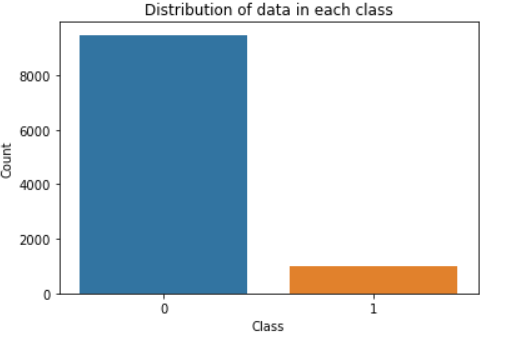
\includegraphics[width=0.5\textwidth]{DataDistribution.png}
\caption{Classes Distribution for Binary Classification problem (Subtask 1)}
\label{fig1}
\end{figure}

\begin{figure}[h]
\centering
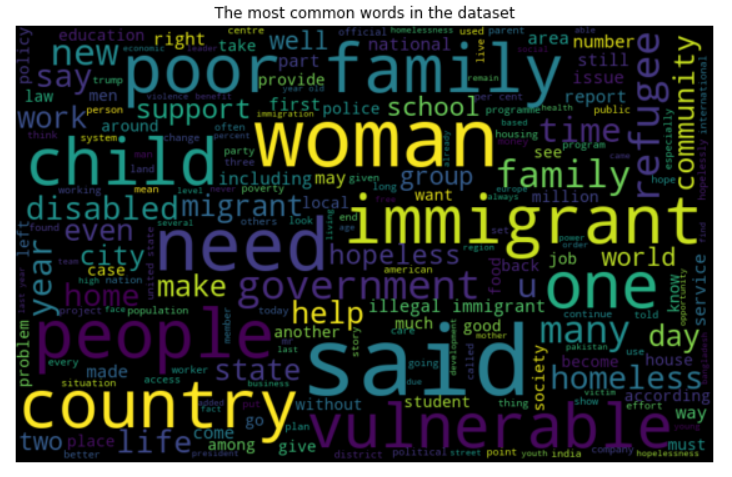
\includegraphics[width=0.5\textwidth]{common.png}
\caption{Most common words in the dataset (Subtask 1)}
\label{fig2}
\end{figure}

\begin{figure}[h]
\centering
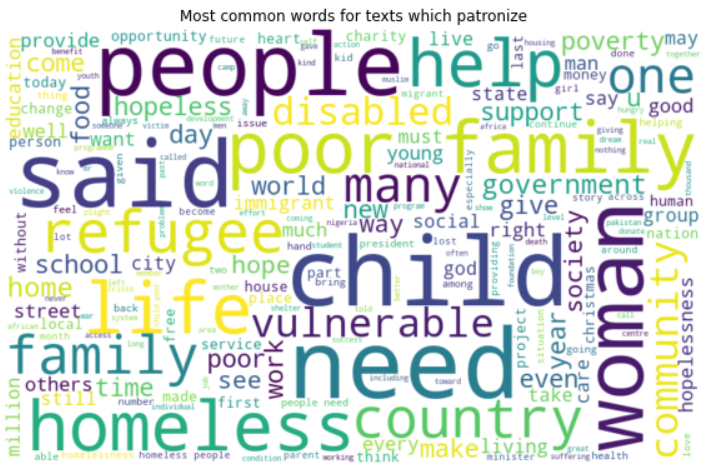
\includegraphics[width=0.5\textwidth]{pcl.png}
\caption{Most common words classified into PCL}
\label{fig3}
\end{figure}

\begin{figure}[h]
\centering
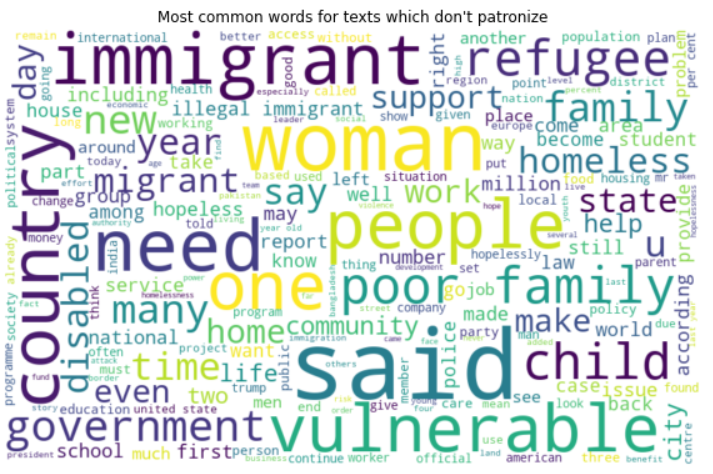
\includegraphics[width=0.5\textwidth]{nopcl.png}
\caption{Most common words of texts that are not PCL}
\label{fig4}
\end{figure}


% TODO:

For taks 2, the paragraphs from task 1 are split according to the type of PCL speech category into sentences, resulting in 950 samples.

\section{System Overview}

\begin{enumerate}
\item Subtask 1 (Binary Classification)

Because the dataset was very imbalanced, we tried different approaches in
order to make it balanced:

\begin{itemize}
\item Adding a class weight to the models used. In this approach, we
computed a metric in which we obtained a class weight according to the
imbalance of the dataset. Through this method, we gave some different
weights to both the majority and minority classes. This whole process had
the purpose to penalize the misclassification made by the minority class by
setting a higher class weight and at the same time, reducing the weight for
the majority class.

\item Using oversampling methods and special ensemble techniques. In this
approach, there were used methods like SMOTE (Synthetic Minority
Over-sampling Technique), Adasyn (Adaptive Synthetic), SVM-SMOTE and self
paced ensemble that performs strictly balanced under-sampling in each
iteration, being very efficient computationally.

\item Augmenting the data. Because we notice so little data for label 1, we
decided to collect hate speech datasets and add the positive texts into our
dataset in order to balance the classes frequency, obtaining a total of 6372
from 795 initial texts with label 1. We'll notice in the results section
that this collection and generation of new dataset didn't provide good
results.
\end{itemize}

The dataset was a little bit preprocessed and split into two preprocessed
types: lemmatized cleaned dataset and stemmed cleaned dataset. These two
datasets were generated in order to make some comparison between those two
techniques and to see which provided the best results.

As feature extraction techniques, there were used techniques like Bag of
Words, Tokenizer, Word2Vec and, finally, BertTokenizer which provided the
best results in the end.

As models, there were used Neural Networks with 3 dense layers, Long Short
Term Memory (LSTM) with 64 and 128 neurons with dropout as well, basic
Machine Learning algorithms like Logistic Regression, Random Forest, Support
Vector Machines as XGBoost. In the end, we decided to try BERT embeddings
and a classification BERT model, BertForSequenceClassification, that
contains a single linear classification layer on top and that provided the
best results after all of the other approaches.

Another approach, called "Text shards" made use of the subtask related to
multiclass classification as well. For an average text that contains PCL,
only some small pieces of them are actually PCL and the rest of the text are
not. The assumption is that this confuses the model, because a a combination
of pcl and non pcl is labeled as PCL. To address this, the following
approach is used:

\begin{itemize}
\item negative examples are left as they are

\item each positive example is replaced with the actual pieces of PCL inside
it that we can get from the categories file

\item the positive examples obtained this way are added with the negative
examples to obtain a training dataset

\item all the sentences are cleaned of characters that are not letters and
the words in each sentence are lemmatized

\item a Tensorflow Hub pretrained model called Universal Sentence Encoder is
trained on it

\item for each text that we want to predict, we first use the model on the
whole text to get an initial label

\item a window (of the size of the average length of a cleaned PCL fragment
* 2) is slided through the text and the model is used to predict that
particular substring. If it is labeled as PCL, then we consider the whole
text as PCL.
\end{itemize}

\item Subtask 2 (Multiclass Classification)

Considering the fact that the vocabulary of the is English only, we have tried
to leverage power of pretrained language models. Therefore we have chosen 3
bert-based models which were pretrained for hatespeech detection and sentiment analysis:

\begin{itemize}

    \item Bert HateXplain \cite{mathew2020hatexplain}: This model was trained to classify text as Hatespeech, Offensive or Normal.
        It was trained on Gab, Twitter and Humain Rationale;
    \item Distil Bert \cite{?}: This model is a version of Distilled bert finetuned on the Twitter dataset;
    \item Distill RoBERTa \cite{?}: This model is a verion of Distilled RoBERTa finetuned on the Twitter dataset;

\end{itemize}

% TODO:

\end{enumerate}

% \section{Experimental setup}

% % TODO:

\section{Results}

\begin{table}[]
    \centering
    \begin{tabular}{scale=.9\linewidth}
        \hline
        Model & UPR & SHA & PRE & AUT  \\
        \hline
        Bert & 0.82 & 0.0 & 0.0 & 0.0 \\
        \hline
        DistilRoberta & 0.83 & 0.0 & 0.0 & 0.0 \\
        \hline
        DistilBert & 0.79 & 0.0 & 0.0 & 0.0 \\
        \hline
        \hline
        Model &  MET & COM & TPTM & F1-Mean \\
        \hline
        Bert &  0.0 & 0.0 & 0.64 & 0.0 \\
        \hline
        DistilRoberta &  0.0 & 0.0 & 0.59 & 0.0 \\
        \hline
        DistilBert &  0.0 & 0.12 & 0.64 & 0.0 \\
        \hline
    \end{tabular}
    \caption{F1 Scores across the categories}
    \label{tab:results}
\end{table}

% TODO:



\section{Conclusion}

% TODO:

\bibliography{custom}

% TODO:

\appendix

\section{Example Appendix}

\label{sec:appendix}

This is an appendix.

\end{document}
